\chapter{Asking Billionaires If Getting Rich Was Worth It}

This lecture is organized as an experiment. We are not given a theorem and then a proof; instead we are given a fixed question and a sequence of test cases. The question is whether the scale of wealth and the sacrifice required to get it are actually worth it, and the lecture answers that question by moving through four billionaire interviews, each of which adds one more ingredient: work, family, challenge, integrity, civic obligation, inner life, leverage, and persistence. The mathematics is therefore not blackboard mathematics, but the arithmetic of exits, returns, debt, scale, and mechanism. We will keep that arithmetic explicit, because it is one of the ways the lecture disciplines its own claims.

\section{Opening Setup: Access, Secrecy, and the Governing Question}

The lecture opens with a small obstruction. Filming is disallowed, privacy is invoked, and then a guard quietly points the interviewer toward a billionaire who has just arrived. That opening is a cold open in the literal sense: it gives us atmosphere before it gives us doctrine. Wealth appears here as something guarded, proximate, and difficult to approach.

The host then resets the frame. He has already interviewed many billionaires about how they got rich, but now he sharpens the problem. The new question is not how to build a large company; it is whether getting rich was worth the cost, and whether money can actually buy happiness. The lecture can be summarized, in a deliberately schematic way, by saying that it refuses to identify wealth with happiness:

\begin{equation}
H \not\equiv H(W).
\end{equation}

Here \(W\) denotes wealth and \(H\) denotes happiness. The point is not that the lecture produces a genuine functional theory of happiness. It does not. The point is that it begins by warning us that any attempt to write such a function in the naive form \(H=H(W)\) is already too crude.

The empirical design is simple. The host will hold the question fixed and vary the interviewee. He moves across two wealthy hubs, Beverly Hills and Las Vegas, and across several kinds of fortune: beverage exits, mobile-phone retail, entertainment entrepreneurship, and finance. The gain from this structure is that the chapter does not have to guess what wealth means in the abstract. We can watch the meaning of wealth change as the cases change.

\section{Beverage Wealth, Work, and Shared Upside}

The first sustained case concerns the builder of major beverage brands. The lecture first establishes scale, and it does so before it asks any philosophical question. BodyArmor is said to have been sold to Coca-Cola for over five billion dollars, and the founder says that on the day of sale he personally made about half a billion dollars. The distinction between company value and personal proceeds is important, and we keep it explicit:

\begin{align}
V_{\text{sale, BodyArmor}} &\approx 5 \times 10^{9}\ \mathrm{USD},\\
P_{\text{founder}} &\approx 5 \times 10^{8}\ \mathrm{USD},\\
\frac{P_{\text{founder}}}{V_{\text{sale, BodyArmor}}} &\approx 0.10.
\end{align}

This last ratio is editorial arithmetic, not a stated cap-table theorem. But it is useful. The lecture keeps reminding us that a huge company outcome and a huge personal outcome are not the same quantity.

What follows is striking because the interviewee does not speak like a man trying to escape work. He is sixty-eight, still building companies, still swimming daily, still speaking in the language of winning. He says he does not really think of himself as working; he thinks of himself as doing what he loves. The lecture therefore begins to dissociate happiness from leisure. For this speaker, ongoing effort is not the negation of happiness; it is one of its preconditions.

Family and employees enter immediately afterward. He has a family, a team, and more than five hundred employees. He says the firm is driven by one goal, namely to win. When asked whether he takes care of his people, he says yes without hesitation, and the examples are deliberately broad: senior executives, assistants, warehouse workers. The point is that shared upside is not presented as an afterthought but as part of the meaning of the success itself.

\subsection{Question \& Answer}

\paragraph{Question.} Does money actually lead to happiness?

\paragraph{Answer.} The first answer is a qualified yes, but only after the lecture has weakened the question. The beverage founder says he is ecstatic, yet in the same breath he says that money is not the answer to everything. The structure of his answer is that wealth amplifies a good life already populated by family, work, and a team whose members also got rich. In this first case, then, money helps, but not as an isolated substance. It helps when it is embedded in contribution, activity, and shared victory.

The host's recap presses precisely this point. He does not summarize the interview by saying simply that money does not matter. He says, rather, that the man made many other people rich, and that there is something in that pattern which feeds both wealth and happiness. The lecture is not yet proving that claim, but it is already treating happiness as socially mediated.

\section{Returns, Repeat Capital, and the Logic of Speed}

The lecture remains with the same case long enough to reveal the mechanism under the headline numbers. First comes a striking investment story. Kobe Bryant, we are told, was not paid to endorse the business. He invested in it.

\paragraph{Worked example: the Kobe Bryant multiple.} The transcript gives an initial investment of six million dollars and then gives two terminal values in different places, one of \(415\) million dollars and another of \(450\) million dollars. We therefore compute a range rather than a single number:
\begin{align}
I_{\text{Kobe}} &= 6 \times 10^{6}\ \mathrm{USD},\\
V_{\text{Kobe}} &\in \left\{4.15 \times 10^{8},\,4.50 \times 10^{8}\right\}\ \mathrm{USD},\\
M_{\text{Kobe}} &= \frac{V_{\text{Kobe}}}{I_{\text{Kobe}}}
\approx 69.2 \text{ to } 75.
\end{align}

\begin{remark}
The lecture later adds that Bryant also received talent-marketing shares. For that reason the range above should be read as a cautious multiple on the stated cash investment, not as a full accounting identity for every component of the final payoff.
\end{remark}

The interview then moves from one deal to the next. The speaker's advice is to surround oneself with good people, make the first deal work, and then carry the winners from the first deal into the second, and from the second into the third. This is not written on a board, but it is a genuine update rule in the logic of entrepreneurship: success creates both cash and trust, and trust lowers the friction of the next raise. When he says he could raise one hundred million dollars in a day if he started another company, that is the numerical expression of reputation compounding.

\begin{equation}
C_{\text{raise}} \approx 1 \times 10^{8}\ \mathrm{USD/day}.
\end{equation}

The lecture then condenses the competitive logic even further through a maxim attributed through Vince Lombardi: it is not the big that eat the small, it is the fast that eat the slow. This line matters because it shifts the chapter from scale to tempo. A firm can be large and still lose; what counts is speed of action. In the lecture's own idiom, if one sits on one's hands, competition runs one over. So the first case gives us more than a happy billionaire. It gives us a mechanism: shared upside, repeat capital, and speed.

\section{The UK Builder: Challenge, Integrity, and Public Obligation}

The second major case moves to a UK entrepreneur whose business was mobile phones in every layer: service provision, retail, distribution, and wholesale. The lecture again begins with scale. He says he built the business from one man in 1986 to twelve thousand people in 2006, and sold it for 1.5 billion pounds.

\begin{equation}
N_{\text{employees}} : 1 \longrightarrow 12{,}000
\qquad (1986\text{--}2006),
\end{equation}

\begin{equation}
V_{\text{exit, UK}} = 1.5 \times 10^{9}\ \mathrm{GBP}.
\end{equation}

What is different in this case is that the speaker narrates his life through challenge rather than through comfort. As a young man he did not know he would become a billionaire. What he had instead was a childhood dream of success, wealth, and charity. When asked whether he is happy, he answers by describing happiness as relative and by tying it to difficult achievement. He gives as example an almost impossible cycling challenge in the Alps. This is important. The lecture is now moving from happiness as the fruit of good relations to happiness as the fruit of hard effort against resistance.

\subsection{Question \& Answer}

\paragraph{Question.} What should wealth do once it has been made?

\paragraph{Answer.} In this second case, wealth must not merely accumulate; it must answer to challenge, truth, and public obligation. The speaker says he is happy when he achieves challenges, but not content. He then says that the deeper business principle is integrity: keep your word, tell the truth, do not sell fantasy as fact. Finally, when the tax question arrives, he rejects the easy offshore path and says that the country in which the money was made should receive the tax. Wealth, in this case, is justified not by comfort but by disciplined use.

The sales discussion is one of the strongest analytical moments in the lecture. The speaker says that when customers asked about early mobile phones, he told them they were dreadful. Others promised perfection; he promised trouble. And because he spoke the truth, he gained credibility. The important mechanism is that truth here is not opposed to selling. Truth is the condition under which selling becomes durable. One could almost say that the lecture treats credibility as a form of invisible capital accumulated by honesty.

The tax discussion pushes the same structure into politics. The speaker says that he paid around two hundred million in taxes and could have avoided that by moving to Monaco.

\begin{equation}
T_{\text{tax}} \approx 2 \times 10^{8}.
\end{equation}

The units are not perfectly stabilized in the transcript, and we therefore keep the numerical claim cautious. But the counterfactual is perfectly clear: move and minimize, or stay and pay. His answer is that one should pay in the country where the money was made. That answer matters because it widens the lecture's moral horizon. Wealth is not now judged only by the owner's life; it is judged by the owner's relation to society.

\section{Delusion, Emptiness, and the Human Experience}

At this point the lecture briefly detours into a pitch for a live event. The interruption is awkward, but it does reveal something methodologically useful: the host sees these interviews not merely as spectacle but as a transfer mechanism by which entrepreneurial knowledge travels from wealthy operators to viewers. It is best treated as a short interruption and not as one of the conceptual pillars of the chapter.

The next major case is Scooter Braun, and the tone changes again. Here the lecture does not begin with mature scale but with youthful delusion. He says that when he began, he was so young that he did not know what could not be done. Great entrepreneurs, he suggests, are a little unrealistic, even delusional. If an idea were fully realistic, it would likely not be great.

The lecture then descends into early scarcity. He recalls a point at which he could not afford a Domino's pizza and had to pay with loose change from a jar shared with roommates. The story matters because it prevents the lecture from turning success into a smooth curve. Success and failure, he says, live next door to one another. That sentence is one of the hidden structural claims of the episode: the distance between visible success and private fragility can be very small.

He then describes a shift in target. At first he wanted a billion dollars. Later he revised the goal downward to ten million, because that seemed enough to support the kind of life he admired. When he passed that number, however, he felt emptiness rather than completion. This is one of the most instructive moments in the lecture: the target was reached, and the payoff was not what had been imagined.

\subsection{Question \& Answer}

\paragraph{Question.} If the target number is reached, why can life still feel empty?

\paragraph{Answer.} Because the lecture has already been warning us that money is not the same object as meaning. Braun says that life comes in ebbs and flows, that every person is having a human experience regardless of wealth, and that inner work cannot be deferred until some enormous fortune appears. The deeper claim is that money can either burden us or free us. It becomes freedom only if we already know what sort of life we are trying to be free for.

This answer is not anti-money. Quite the contrary. The lecture keeps the full force of money in view. Money can set one free to spend more time with friends, help other entrepreneurs, give away tickets, and enlarge the field of life. But that freedom is not self-interpreting. Without self-knowledge, scale remains structurally empty. The chapter must preserve this point carefully, because it is easy to flatten it into vague self-help. What the lecture actually says is more precise: wealth is powerful, but inner disorder survives wealth.

\section{Leverage, Debt, and the Scale of Wealth}

The final major case in Las Vegas begins with more search, more refusals, more partial access, and then a breakthrough into a finance-and-private-equity conversation. If the earlier interviews asked what wealth feels like from the inside, this last one most clearly asks how wealth scales.

The speaker first gives a large paper-gain number from taking a company public, and then compresses the lesson into the cleanest formal structure of the whole lecture: there are only three ways to make money, by leveraging people, time, or money. This deserves to be written cleanly.

\begin{definition}
The lecture's leverage triad is
\begin{equation}
\mathcal{L}=\{L_p,L_t,L_m\}
=\{\text{people},\ \text{time},\ \text{money}\}.
\end{equation}
Here \(L_p\) denotes leverage through other people's labor or skill, \(L_t\) denotes leverage through time, and \(L_m\) denotes leverage through capital.
\end{definition}

The lecture does not offer a formal production function, but its implicit scaling claim can be written schematically as
\begin{equation}
W_{\text{scale}} \sim F(L_p,L_t,L_m).
\end{equation}
This is not meant as a rigorous model. It is a compact way of preserving the speaker's point that wealth at scale comes from moving beyond the sale of one's own labor-time alone.

\begin{figure}[h]
\centering
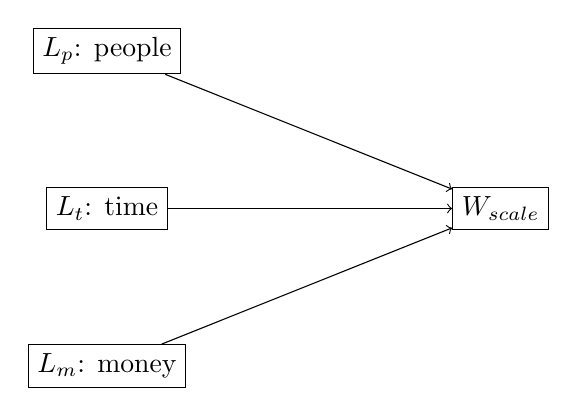
\begin{tikzpicture}
\node[draw] (p) at (0,2) {$L_p$: people};
\node[draw] (t) at (0,0) {$L_t$: time};
\node[draw] (m) at (0,-2) {$L_m$: money};
\node[draw] (w) at (5,0) {$W_{\text{scale}}$};
\draw[->] (p) -- (w);
\draw[->] (t) -- (w);
\draw[->] (m) -- (w);
\end{tikzpicture}
\end{figure}

The lawyer example is useful here. If one works only as a lawyer for someone else, one is mainly selling time. One may live comfortably, but the scale is bounded. If one starts a firm and has many lawyers working under the same roof, one begins to leverage people as well as time. If one can deploy capital itself, one adds a third channel. The lecture's mechanism is not mysterious. It is a hierarchy of leverage.

\subsection{Question \& Answer}

\paragraph{Question.} How does wealth actually scale?

\paragraph{Answer.} The lecture's last answer is that wealth scales when the unit of activity stops being merely one's own hours. It scales through people, through organized time, through capital, and through the ability to hire complementary skill. But the lecture does not leave the matter there. It immediately re-embeds leverage in biography: deep debt, a mentor who stayed, many books, marriage, children, faith, and a refusal to quit. Scale is thus technical and human at once.

This last point matters. The speaker says he had once been deeply in debt, had borrowed money from his mother, and had lived through depression. He then says that one needs mentors and one needs books. The lecture therefore closes where it began: not with a machine that prints wealth, but with a person who must cross uncertainty, persist through failure, and learn how to convert experience into structure.

\section{Summary}

The lecture never gives us a single final formula for happiness, and that is one of its virtues. Instead it gives us a sequence of increasingly refined refusals. Wealth is not identical to happiness. Leisure is not identical to happiness. Retirement is not identical to happiness. A target number is not identical to happiness. What the lecture does allow us to say is that wealth changes the scale of action, the size of the field, and the number of options. But whether that expanded field becomes a good life depends on mediating structures: family, contribution, challenge, truthfulness, civic obligation, self-knowledge, and the ability to leverage skill without losing one's humanity.

So the chapter ends as the lecture ends: not with a theorem that money buys happiness, and not with the opposite theorem that money is irrelevant, but with a harder claim. Money matters enormously. It is simply not the last variable.